\everymath{\displaystyle}

%%%%%%%%%%%%%%%%%%%%%%%%%%%%%%%%%%%%%%%%
%           main body
%%%%%%%%%%%%%%%%%%%%%%%%%%%%%%%%%%%%%%%%

%-----------------------------------
%	TITLE PAGE
%-----------------------------------

\title[第十章\\
函数项级数]{\texorpdfstring{\LARGE \bfseries 第十章\quad 函数项级数}{第十章 函数项级数}} % The short title appears at the bottom of every slide, the full title is only on the title page
\author[\smaller \S 10.2\\
一致收敛级数的判别和性质] % Your institution as it will appear on the bottom of every slide, maybe shorthand to save space
{\Large \bfseries \S 10.2 一致收敛级数的判别和性质}
% \author{Singular Value Decomposition} % Your name
% \date{\today} % Date, can be changed to a custom date
\date{}

%------------------------------------------------

\begin{document}

%------------------------------------------------

\begin{frame}

\titlepage % Print the title page as the first slide

\end{frame}

%-----------------------------------
%	PRESENTATION SLIDES
%-----------------------------------

%------------------------------------------------

\begin{frame}
\frametitle{绪言}

我们已有的基于``距离'', 或是基于数列的极限的函数项级数的一致收敛性的判别方法, 都首先需要将函数项级数的和函数或者函数列的极限函数求出来. 这对于仅仅需要判断一致收敛性的情况来说, 是不必要的, 而且在某些情况下甚至是不可行的. 于是我们需要一些不需要求出和函数或者极限函数的表达式, 就可以判断一致收敛性的判别方法. 这一节我们将介绍一些这样的判别方法.

\pause
\vspace{1em}

我们已经介绍过这样一种基本的方法了:

\begin{thm}[Cauchy 收敛原理]
函数项级数 $\displaystyle \sum_{n=0}^\infty u_n(x)$ 在 $D$ 上一致收敛的充分必要条件是: 对任意 $\varepsilon > 0,$ 存在只与 $\varepsilon$ 有关的正整数 $N(\varepsilon)$, 使得当 $m > n \geqslant N(\varepsilon)$ 时, 对任意 $x \in D,$ 都有
\begin{equation*}
\left| \sum_{k=n+1}^m u_k(x) \right| = \left| u_{n+1}(x) + u_{n+2}(x) + \cdots + u_m(x) \right| < \varepsilon.
\end{equation*}
\end{thm}

\end{frame}

%------------------------------------------------

\begin{frame}
\frametitle{绪言}

\begin{remark}
\begin{itemize}
\item 相应地, 函数列 $\{S_n(x)\}$ 在 $D$ 上一致收敛的 Cauchy 收敛原理是: 对任意 $\varepsilon > 0,$ 存在只与 $\varepsilon$ 有关的正整数 $N(\varepsilon)$, 使得当 $m > n \geqslant N(\varepsilon)$ 时, 对任意 $x \in D,$ 都有 $S_m(x) - S_n(x) < \varepsilon.$
\item Cauchy 收敛原理对一般的完备的度量空间中元素的序列 (族) 的收敛性判别同样适用.
\end{itemize}
\end{remark}

\pause
\vspace{1em}

Cauchy 收敛原理虽然是函数项级数一致收敛性的一个充分必要条件, 但是在实际应用中, 由于需要对任意 $m > n \geqslant N(\varepsilon)$ 和任意 $x \in D$ 都满足的条件进行验证, 因此使用起来非常麻烦. 下面我们将介绍一些更为实用的判别方法.

\end{frame}

%------------------------------------------------

\section{一致收敛的判别}

%------------------------------------------------

\begin{frame}
\frametitle{Weierstraß 判别法}

类似于正项级数的比较判别法, 函数项级数也有类似的判别方法, 最简单的情况就是被比较的函数项级数是一个正项级数, 这就是所谓的 Weierstraß 判别法:

\begin{thm}[Weierstraß 判别法]
设 $\{u_n(x)\}$ 是定义在 $D$ 上的函数列, $\{a_n\}$ 是正数列, 满足 $|u_n(x)| \leqslant a_n$ 对任意 $n \in \mathbb{N}$ 和 $x \in D$ 都成立. 如果正项级数 $\displaystyle \sum_{n=0}^\infty a_n$ 收敛, 那么函数项级数 $\displaystyle \sum_{n=0}^\infty u_n(x)$ 在 $D$ 上一致收敛.
\end{thm}

\pause
\vspace{0.5em}

\begin{eg}
设数项级数 $\sum_{n=1}^\infty a_n$ 绝对收敛, 那么由 Weierstraß 判别法, 函数项级数
\[
\sum_{n=1}^\infty a_n \sin (n x), ~~ \sum_{n=1}^\infty a_n \cos (n x)
\]
在 $\mathbb{R}$ 上一致收敛.
\pause
例如, $a_n = \frac{1}{n^s}, s > 1;$ $a_n = \frac{(-1)^{n+1}}{n^2 + 1}$ 等等.
\end{eg}

\end{frame}

%------------------------------------------------

\begin{frame}
\frametitle{Weierstraß 判别法的应用}

\begin{eg}
讨论函数项级数 $\displaystyle \sum_{n=1}^\infty u_n(x) = \sum_{n=1}^\infty x^\alpha e^{-nx}$ 在 $D = [0, +\infty)$ 上的收敛性, 其中 $\alpha \in \mathbb{R}$ 是一个参数.
\end{eg}

\pause
\vspace{0.5em}

\startproof[bg=yellow, fg=red](解)
首先, 由正项级数的 Cauchy 判别法, 对所有固定的 $x \in D$ 以及 $\alpha \in \mathbb{R},$ 数项级数
\[
\sqrt[n]{u_n(x)} = \sqrt[n]{x^\alpha e^{-nx}} = x^{\alpha/n} e^{-x} \to e^{-x} < 1, ~~ n \to \infty,
\]
所以函数项级数 $\displaystyle \sum_{n=1}^\infty u_n(x)$ 的收敛域 (逐点收敛) 就是 $D = [0, +\infty).$ 下面我们来讨论函数项级数 $\displaystyle \sum_{n=1}^\infty u_n(x)$ 在 $D$ 上的一致收敛性.

\pause
\vspace{0.5em}

{\color{red}\ding{43}} 对于 $\alpha \leqslant 0$ 的情况, 很容易观察到
\[
\lim_{x \to 0^+} u_n(x) = \lim_{x \to 0^+} x^\alpha e^{-nx} = +\infty,
\]
不满足一致收敛的必要条件, 所以 $\alpha \leqslant 0$ 时函数项级数 $\displaystyle \sum_{n=1}^\infty u_n(x)$ 在 $D$ 上不一致收敛.

\end{frame}

%------------------------------------------------

\begin{frame}
\frametitle{Weierstraß 判别法的应用}

{\color{red}\ding{43}} 对于 $\alpha > 0$ 的情况, 有两个比较重要的观察:
\begin{itemize}
\item 对所有 $\alpha \in \mathbb{R}$ 有 $\lim_{x\to +\infty} u_n(x) = \lim_{x\to +\infty} x^\alpha e^{-nx} = 0.$
\item 对所有 $\alpha > 0$ 有 $\lim_{x\to 0^+} u_n(x) = \lim_{x\to 0^+} x^\alpha e^{-nx} = 0.$
\end{itemize}
于是, 对所有 $\alpha > 0,$ $\exists M_n(\alpha) \in \mathbb{R}^+$ 使得 $M_n(\alpha) = \max_{x \in D} u_n(x).$
\pause
可以进一步求出这个值: 对 $u_n(x)$ 关于 $x$ 求导, 有
\[
u_n'(x) = \alpha x^{\alpha - 1} e^{-nx} - n x^\alpha e^{-nx} = x^{\alpha - 1} e^{-nx} (\alpha - nx).
\]
所以 $u_n(x)$ 在 $x = \frac{\alpha}{n}$ 处取得最大值, 从而 $M_n(\alpha) = u_n\left( \frac{\alpha}{n} \right) = \left( \frac{\alpha}{e} \right)^\alpha \cdot \frac{1}{n^\alpha}.$

\pause
\vspace{0.5em}

{\color{red}\ding{43}} 对于 $\alpha > 1$ 的情况, 由于正项级数 $\sum_{n=1}^\infty M_n(\alpha)$ 收敛, 由 Weierstraß 判别法, 函数项级数 $\displaystyle \sum_{n=1}^\infty u_n(x)$ 在 $D$ 上一致收敛.

\pause
\vspace{0.5em}

{\color{red}\ding{43}} 对于 $0 < \alpha \leqslant 1$ 的情况, 由于 $\sum_{n=1}^\infty M_n(\alpha)$ 发散, 不能直接使用 Weierstraß 判别法, 需要另外想办法进行判断.

\end{frame}

%------------------------------------------------

\begin{frame}
\frametitle{Weierstraß 判别法的应用}

\begin{columns}
\begin{column}{0.4\textwidth}
\begin{center}
\scalebox{0.9}{
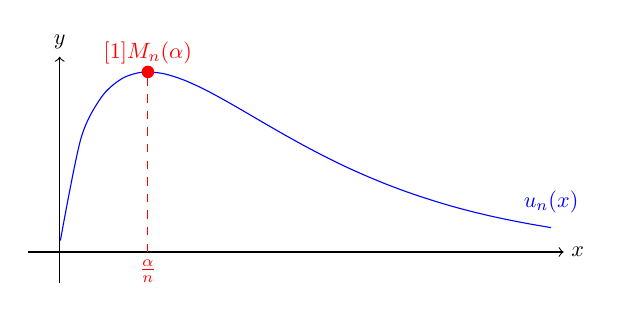
\begin{tikzpicture}[scale=0.8, every node/.append style={scale=0.8}]
\def\nValue{2}
\def\alphaValue{0.7}
\draw[->] (-0.5, 0) -- (8, 0) node[right] {$x$};
\draw[->] (0, -0.5) -- (0, 3.1) node[above] {$y$};
% scale x, y for better visualization
\def\yscaleValue{12}
\def\xscaleValue{4}
% plot u_n(x) with marked M_n(\alpha)
\draw[domain=0.01:7.8, smooth, variable=\x, blue] plot ({\x}, {\yscaleValue * (\x / \xscaleValue)^\alphaValue * exp(-\nValue * (\x / \xscaleValue))});
\node[color=blue] at (7.8, 0.5) [above] {$u_n(x)$};
% marked M_n(\alpha)
\draw[dashed, red] ({\xscaleValue*\alphaValue/\nValue}, 0) node[below] {$\frac{\alpha}{n}$} -- ({\xscaleValue*\alphaValue/\nValue}, {\yscaleValue * (\alphaValue/\nValue)^\alphaValue * exp(-\nValue * (\alphaValue/\nValue))}) node[above] {\smaller[1]$M_n(\alpha)$} node[circle, fill=red, inner sep=2pt] {};
\end{tikzpicture}
}
\end{center}
\end{column}
\begin{column}{0.6\textwidth}
由于 $M_n(\alpha) = \left( \frac{\alpha}{e} \right)^\alpha \cdot \frac{1}{n^\alpha} \to 0 ~ (n \to \infty),$ 所以\alert{不可以}通过选取数列 $\{x_n\}$ 使得 $u_n(x_n) \nrightarrow 0$ 从而得出 $u_n(x)$ 不一致收敛到 $0,$ 进而得出函数项级数 $\displaystyle \sum_{n=1}^\infty u_n(x)$ 在 $D$ 上不一致收敛的结论.
\end{column}
\end{columns}

\pause

\begin{columns}
\begin{column}{0.4\textwidth}
\begin{center}
\scalebox{0.9}{
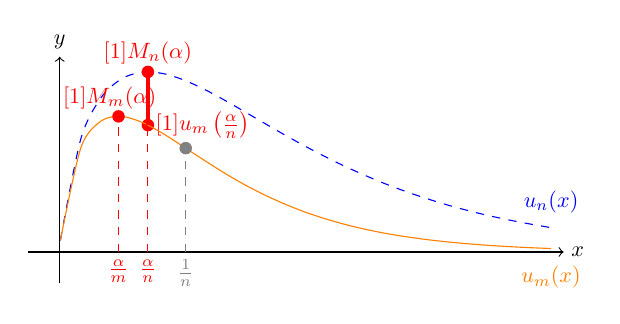
\begin{tikzpicture}[scale=0.8, every node/.append style={scale=0.8}]
% plot u_n(x) with marked M_n(\alpha)
\def\nValue{2}
\def\mValue{3}
\def\alphaValue{0.7}
\draw[->] (-0.5, 0) -- (8, 0) node[right] {$x$};
\draw[->] (0, -0.5) -- (0, 3.1) node[above] {$y$};
% scale x, y for better visualization
\def\yscaleValue{12}
\def\xscaleValue{4}
% draw u_n(x)
\draw[domain=0.01:7.8, smooth, variable=\x, blue, dashed] plot ({\x}, {\yscaleValue * (\x / \xscaleValue)^\alphaValue * exp(-\nValue * (\x / \xscaleValue))});
\node[color=blue] at (7.8, 0.5) [above] {$u_n(x)$};
% vertical dashed line at x = alpha/n with marked M_n(\alpha) and u_m(alpha/n)
\draw[dashed, red] ({\xscaleValue*\alphaValue/\nValue}, 0) node[below] {$\frac{\alpha}{n}$} -- ({\xscaleValue*\alphaValue/\nValue}, {\yscaleValue * (\alphaValue/\nValue)^\alphaValue * exp(-\nValue * (\alphaValue/\nValue))}) node[above] {\smaller[1]$M_n(\alpha)$} node[circle, fill=red, inner sep=2pt] {};
\node[circle, fill=red, inner sep=2pt] at ({\xscaleValue*\alphaValue/\nValue}, {\yscaleValue * (\alphaValue/\nValue)^\alphaValue * exp(-\mValue * (\alphaValue/\nValue))}) {};
\node[color=red, right] at ({\xscaleValue*\alphaValue/\nValue}, {\yscaleValue * (\alphaValue/\nValue)^\alphaValue * exp(-\mValue * (\alphaValue/\nValue))}) {\smaller[1]$u_m\left(\frac{\alpha}{n}\right)$};
% draw u_m(x) for comparison
\draw[domain=0.01:7.8, smooth, variable=\x, orange] plot ({\x}, {\yscaleValue * (\x / \xscaleValue)^\alphaValue * exp(-\mValue * (\x / \xscaleValue))});
\node[color=orange] at (7.8, -0.1) [below] {$u_m(x)$};
% vertical dashed line at x = alpha/m with marked M_m(\alpha)
\draw[dashed, red] ({\xscaleValue*\alphaValue/\mValue}, 0) node[below] {$\frac{\alpha}{m}$} -- ({\xscaleValue*\alphaValue/\mValue}, {\yscaleValue * (\alphaValue/\mValue)^\alphaValue * exp(-\mValue * (\alphaValue/\mValue))}) node[above, xshift=-4pt] {\smaller[1]$M_m(\alpha)$} node[circle, fill=red, inner sep=2pt] {};
% vertical dashed line at x = 1/n with marked u_n(1/n)
\draw[dashed, gray] ({\xscaleValue/\nValue}, 0) node[below] {$\frac{1}{n}$} -- ({\xscaleValue/\nValue}, {\yscaleValue * (1/\nValue)^\alphaValue * exp(-\mValue * (1/\nValue))}) node[circle, fill=gray, inner sep=2pt] {};
% draw red line segment between (alpha/n, u_m(alpha/n)) and M_n(\alpha) to show the distance
\draw[color=red, ultra thick] ({\xscaleValue*\alphaValue/\nValue}, {\yscaleValue * (\alphaValue/\nValue)^\alphaValue * exp(-\mValue * (\alphaValue/\nValue))}) -- ({\xscaleValue*\alphaValue/\nValue}, {\yscaleValue * (\alphaValue/\nValue)^\alphaValue * exp(-\nValue * (\alphaValue/\nValue))});
\end{tikzpicture}
}
\end{center}
\end{column}
\begin{column}{0.6\textwidth}
希望证明 $\sum_{n=1}^\infty u_n(x)$ 不一致收敛, 可以利用 Cauchy 收敛原理的反面, 即选取一些特定的可以任意大的 $m, n,$ 以及特定的 $x \in D,$ 使得 $\left| \sum_{k=n+1}^m u_k(x) \right|$ 足够大.
\pause
现在考察 $x = \frac{\alpha}{n}$ 时的情况. 对于 $m > n,$ 考察 $u_m\left(\frac{\alpha}{n}\right) = \left( \frac{\alpha}{n} \right)^\alpha e^{-\frac{m}{n} \alpha}$ 与 $M_n(\alpha) = u_n\left(\frac{\alpha}{n}\right) = \left( \frac{\alpha}{n} \right)^\alpha e^{-\alpha}$ 的距离. 这二者相差不远.
\end{column}
\end{columns}

\end{frame}

%------------------------------------------------

\begin{frame}
\frametitle{Weierstraß 判别法的应用}

\begin{center}
\scalebox{1.0}{
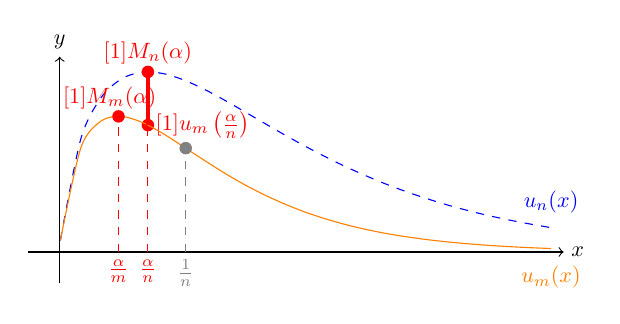
\begin{tikzpicture}[scale=0.8, every node/.append style={scale=0.8}]
% plot u_n(x) with marked M_n(\alpha)
\def\nValue{2}
\def\mValue{3}
\def\alphaValue{0.7}
\draw[->] (-0.5, 0) -- (8, 0) node[right] {$x$};
\draw[->] (0, -0.5) -- (0, 3.1) node[above] {$y$};
% scale x, y for better visualization
\def\yscaleValue{12}
\def\xscaleValue{4}
% draw u_n(x)
\draw[domain=0.01:7.8, smooth, variable=\x, blue, dashed] plot ({\x}, {\yscaleValue * (\x / \xscaleValue)^\alphaValue * exp(-\nValue * (\x / \xscaleValue))});
\node[color=blue] at (7.8, 0.5) [above] {$u_n(x)$};
% vertical dashed line at x = alpha/n with marked M_n(\alpha) and u_m(alpha/n)
\draw[dashed, red] ({\xscaleValue*\alphaValue/\nValue}, 0) node[below] {$\frac{\alpha}{n}$} -- ({\xscaleValue*\alphaValue/\nValue}, {\yscaleValue * (\alphaValue/\nValue)^\alphaValue * exp(-\nValue * (\alphaValue/\nValue))}) node[above] {\smaller[1]$M_n(\alpha)$} node[circle, fill=red, inner sep=2pt] {};
\node[circle, fill=red, inner sep=2pt] at ({\xscaleValue*\alphaValue/\nValue}, {\yscaleValue * (\alphaValue/\nValue)^\alphaValue * exp(-\mValue * (\alphaValue/\nValue))}) {};
\node[color=red, right] at ({\xscaleValue*\alphaValue/\nValue}, {\yscaleValue * (\alphaValue/\nValue)^\alphaValue * exp(-\mValue * (\alphaValue/\nValue))}) {\smaller[1]$u_m\left(\frac{\alpha}{n}\right)$};
% draw u_m(x) for comparison
\draw[domain=0.01:7.8, smooth, variable=\x, orange] plot ({\x}, {\yscaleValue * (\x / \xscaleValue)^\alphaValue * exp(-\mValue * (\x / \xscaleValue))});
\node[color=orange] at (7.8, -0.1) [below] {$u_m(x)$};
% vertical dashed line at x = alpha/m with marked M_m(\alpha)
\draw[dashed, red] ({\xscaleValue*\alphaValue/\mValue}, 0) node[below] {$\frac{\alpha}{m}$} -- ({\xscaleValue*\alphaValue/\mValue}, {\yscaleValue * (\alphaValue/\mValue)^\alphaValue * exp(-\mValue * (\alphaValue/\mValue))}) node[above, xshift=-4pt] {\smaller[1]$M_m(\alpha)$} node[circle, fill=red, inner sep=2pt] {};
% vertical dashed line at x = 1/n with marked u_n(1/n)
\draw[dashed, gray] ({\xscaleValue/\nValue}, 0) node[below] {$\frac{1}{n}$} -- ({\xscaleValue/\nValue}, {\yscaleValue * (1/\nValue)^\alphaValue * exp(-\mValue * (1/\nValue))}) node[circle, fill=gray, inner sep=2pt] {};
% draw red line segment between (alpha/n, u_m(alpha/n)) and M_n(\alpha) to show the distance
\draw[color=red, ultra thick] ({\xscaleValue*\alphaValue/\nValue}, {\yscaleValue * (\alphaValue/\nValue)^\alphaValue * exp(-\mValue * (\alphaValue/\nValue))}) -- ({\xscaleValue*\alphaValue/\nValue}, {\yscaleValue * (\alphaValue/\nValue)^\alphaValue * exp(-\nValue * (\alphaValue/\nValue))});
\end{tikzpicture}
}
\end{center}

那么有
\[
\sum_{k=n+1}^m u_k\left(\frac{\alpha}{n}\right) = \sum_{k=n+1}^m \left( \frac{\alpha}{n} \right)^\alpha e^{-\frac{k}{n} \alpha} \geqslant (m-n) \cdot \left( \frac{\alpha}{n} \right)^\alpha e^{-\frac{m}{n} \alpha}.
\]
若取 $m = pn,$ $p \geqslant 2$ 为固定的整数, 则上式变为
\[
\sum_{k=n+1}^m u_k\left(\frac{\alpha}{n}\right) \geqslant \alpha^\alpha \cdot (p-1) \cdot e^{-\alpha p} \cdot n^{1-\alpha} \to +\infty, ~~ n \to \infty,
\]
这样就证明了对于 $0 < \alpha \leqslant 1$ 的情况, 函数项级数 $\displaystyle \sum_{n=1}^\infty u_n(x)$ 在 $D$ 上不一致收敛.
\qed

\end{frame}

%------------------------------------------------

\begin{frame}
\frametitle{函数项级数一致收敛的 A-D 判别法}

讲完了对应于正项级数比较判别法的 Weierstraß 判别法, 下面我们来介绍对应于任意项级数的 A-D 判别法的函数项级数版本:
\pause
\begin{thm}[A-D 判别法]
设函数项级数 $\displaystyle \sum_{n=0}^\infty a_n(x)b_n(x)$ 收敛域为 $D,$ 如果如下条件之一成立, 则该函数项级数在 $D$ 上一致收敛:
\begin{itemize}
\item Abel 判别法
\begin{itemize}
\item[$1^\circ$] $\{a_n(x)\}$ 对于每个固定的 $x \in D$ 关于 $n$ 单调, 且 $\{a_n(x)\}$ 在 $D$ 上一致有界: 即存在 $M > 0$ 使得 $|a_n(x)| \leqslant M$ 对任意 $n \in \mathbb{N}$ 和 $x \in D$ 都成立;
\item[$2^\circ$] 数项级数 $\displaystyle \sum_{n=0}^\infty b_n(x)$ 在 $D$ 上一致收敛.
\end{itemize}
\item Dirichlet 判别法
\begin{itemize}
\item[$1^\circ$] $\{a_n(x)\}$ 对于每个固定的 $x \in D$ 关于 $n$ 单调, 且 $\{a_n(x)\}$ 在 $D$ 上一致收敛到 $0;$
\item[$2^\circ$] 数项级数 $\displaystyle \sum_{n=0}^\infty b_n(x)$ 在 $D$ 上一致有界.
\end{itemize}
\end{itemize}
\end{thm}

\end{frame}

%------------------------------------------------

\begin{frame}
\frametitle{A-D 判别法的证明}

这里给出 Abel 判别法的证明, Dirichlet 判别法的证明与之类似.

\pause
\vspace{0.5em}

\startproof[bg=yellow, fg=red]
由于 $\displaystyle \sum_{n=0}^\infty b_n(x)$ 在 $D$ 上一致收敛, 由 Cauchy 收敛原理, 对任意 $\varepsilon > 0,$ 存在只与 $\varepsilon$ 有关的正整数 $N(\varepsilon)$, 使得当 $m > n \geqslant N(\varepsilon)$ 时, 对任意 $x \in D,$ 都有
\[
\left| \sum_{k=n+1}^m b_k(x) \right| < \varepsilon / 3M.
\]
记 $B_k(x) = \sum_{j=n+1}^k b_j(x), k = n+1, n+2, \cdots, m,$ 并约定 $B_{n}(x) = 0.$ 那么
\begin{align*}
\sum_{k=n+1}^m a_k(x) b_k(x) & = \sum_{k=n+1}^m a_k(x) (B_k(x) - B_{k-1}(x)) = \sum_{k=n+1}^m a_k(x) B_k(x) - \sum_{k=n+1}^m a_k(x) B_{k-1}(x) \\
& = \sum_{k=n+1}^m a_k(x) B_k(x) - \sum_{k=n}^{m-1} a_{k+1}(x) B_k(x) \\
& = \sum_{k=n+1}^{m-1} (a_k(x) - a_{k+1}(x)) B_k(x) + a_m(x) B_m(x) - a_{n+1}(x) B_{n}(x).
\end{align*}

\end{frame}

%------------------------------------------------

\begin{frame}
\frametitle{A-D 判别法的证明}

于是有
\begin{align*}
\left| \sum_{k=n+1}^m a_k(x) b_k(x) \right| & = \left| \sum_{k=n+1}^{m-1} (a_k(x) - a_{k+1}(x)) B_k(x) + a_m(x) B_m(x) - a_{n+1}(x) B_{n}(x) \right| \\
& \leqslant \frac{\varepsilon}{3M} \left( \sum_{k=n+1}^{m-1} |a_k(x) - a_{k+1}(x)| + |a_m(x)| \right) \\
& {\color{red} =} \frac{\varepsilon}{3M} \left( |a_{n+1}(x) - a_m(x)| + |a_m(x)| \right) \\
& \leqslant \frac{\varepsilon}{3M} \cdot 3M = \varepsilon.
\end{align*}
上式中等号 {\color{red} =} 的成立是由于 $\{a_n(x)\}$ 关于 $n$ 单调, 从而 $a_k(x) - a_{k+1}(x)$ 的符号不变, 使得
\[
\sum_{k=n+1}^{m-1} |a_k(x) - a_{k+1}(x)| = \left| \sum_{k=n+1}^{m-1} (a_k(x) - a_{k+1}(x)) \right| = |a_{n+1}(x) - a_m(x)|.
\]

以上, 我们相当于又把 Abel 引理, 或者说分部求和公式又证明了一遍.
\qed

\end{frame}

%------------------------------------------------

\begin{frame}
\frametitle{应用例题}

\begin{eg}
考察 $\sum_{n=1}^\infty a_n \cos (n x), \sum_{n=1}^\infty a_n \sin (n x)$ 的一致收敛性, 其中 $\{a_n\}$ 是一个数列.
\end{eg}

\pause
\vspace{0.5em}

之前我们已经通过 Weierstraß 判别法得出, 如果数项级数 $\sum_{n=1}^\infty a_n$ 绝对收敛, 那么函数项级数 $\displaystyle \sum_{n=1}^\infty a_n \sin (n x), \sum_{n=1}^\infty a_n \cos (n x)$ 在 $\mathbb{R}$ 上一致收敛. 如果将条件减弱为 $a_n \searrow 0,$ 那么情况如何呢?

\pause
\vspace{0.5em}

可以将 $a_n$ 视为常值函数, 那么可以利用 Dirichlet 判别法, 需要考察 $\sum_{k=1}^n \sin (k x)$ 和 $\sum_{k=1}^n \cos (k x)$ 是否关于 $n$ 对 $x$ 一致有界. 之前已经证明了 (通过和差化积+积化和差, 或者通过复数指数函数的形式),
\[
\sum_{k=1}^n \sin (k x) = \begin{cases}
0, & x = 2m\pi, m \in \mathbb{Z}, \\
\dfrac{\cos\frac{x}{2} - \cos\frac{(2n+1)x}{2}}{2\sin\frac{x}{2}}, & x \neq 2m\pi, m \in \mathbb{Z},
\end{cases}
\]

\end{frame}

%------------------------------------------------

\begin{frame}
\frametitle{应用例题}

所以当 $D = [a, b] \subset (0, 2\pi)$ (或者任意 $(2m\pi, 2(m+1)\pi), m \in \mathbb{Z}$) 时, 有
\[
\left| \sum_{k=1}^n \sin (k x) \right| \leqslant \frac{1}{\left|\sin\frac{x}{2}\right|} \leqslant \max\left\{ \frac{1}{\left|\sin\frac{a}{2}\right|}, \frac{1}{\left|\sin\frac{b}{2}\right|} \right\}, ~~ \forall n \in \mathbb{N}, x \in D.
\]
于是, 函数项级数 $\displaystyle \sum_{n=1}^\infty a_n \sin (n x), \sum_{n=1}^\infty a_n \cos (n x)$ 在每个 $(2m\pi, 2(m+1)\pi), m \in \mathbb{Z}$ 上\alert{内闭一致收敛}.

类似可证 $\displaystyle \sum_{n=1}^\infty a_n \sin (n x), \sum_{n=1}^\infty a_n \cos (n x)$ 在每个 $(2m\pi, 2(m+1)\pi), m \in \mathbb{Z}$ 上内闭一致收敛.
\qed

\end{frame}

%------------------------------------------------

\begin{frame}
\frametitle{应用例题}

\begin{eg}
设数项级数 $\sum_{n=1}^\infty a_n$ 收敛, 考察函数项级数 $\displaystyle \sum_{n=1}^\infty a_n x^n.$
\end{eg}

\vspace{0.5em}

{\color{red}\ding{43}} 问题一: 收敛域 $D$ 是什么?

\pause

首先, 当 $x_0 \in [0, 1]$ 时, $x_0^n$ 单调有界, 那么由数项级数的 Abel 判别法, $\displaystyle \sum_{n=1}^\infty a_n x_0^n$ 收敛, 所以 $[0, 1] \subset D.$
\pause
实际上, 收敛域 $D$ 可能更大, 例如
\begin{itemize}
\item 当 $a_n = \frac{1}{n!},$ 那么 $D = \mathbb{R}.$
\item 当 $a_n = \frac{1}{2^n},$ 那么 $D = (-2, 2).$
\item 当 $a_n = \frac{(-1)^{n+1}}{\ln(n+1)},$ 那么 $D = (-1, 1].$
\end{itemize}

\end{frame}

%------------------------------------------------

\begin{frame}
\frametitle{应用例题}

对于 $x_0 \in (-1, 0),$ 由于数项级数 $\sum_{n=1}^\infty x_0^n$ 绝对收敛, 且 $a_n \to 0,$ 所以容易由 Cauchy 收敛原理得出 $\displaystyle \sum_{n=1}^\infty a_n x_0^n$ 收敛, 从而 $(-1, 0) \subset D.$

\pause

所以, 关于收敛域, 我们得出的结论是 $(-1, 1] \subset D.$

\vspace{0.5em}

{\color{red}\ding{43}} 问题二: $\displaystyle \sum_{n=1}^\infty a_n x^n$ 在 $(-1, 1]$ 上是否 (内闭) 一致收敛?

\pause

对于区间 $[0, 1],$ 由于 $u_n(x) := x^n$ 单调且一致有界, 数项级数 $\displaystyle \sum_{n=1}^\infty a_n$ 收敛, 由 Abel 判别法, $\displaystyle \sum_{n=1}^\infty a_n x^n$ 在 $[0, 1]$ 上一致收敛.

\pause

对于闭区间 $[a, b] \subset (-1, 0],$ $-1 < a < b \leqslant 0,$ 由于 $a_n \to 0,$ 当 $n$ 充分大时, $|a_n| < 1,$ 那么有
\[
\left| \sum_{k=n+1}^m a_k x^k \right| \leqslant \sum_{k=n+1}^m |a_k| \cdot |x|^k \leqslant \sum_{k=n+1}^m |a|^k \to 0, ~~ n \to \infty.
\]
于是, $\displaystyle \sum_{n=1}^\infty a_n x^n$ 在 $(-1, 1]$ 上\alert{内闭一致收敛}.
\qed

\end{frame}

%------------------------------------------------

\section{一致收敛函数项级数 (函数列) 的分析性质}

%------------------------------------------------

\begin{frame}
\frametitle{一致收敛函数项级数 (函数列) 的连续性}

我们要研究的所谓``分析性质'' 包括连续性, 可导性, 可积性等. 首先来看连续性. 以下都考虑函数列.

\pause
\vspace{1em}

\begin{thm}[一致收敛函数列的连续性定理]
设函数列 $\{S_n(x)\}$ 的每一项在 $[a, b]$ 上连续, 且 $\{S_n(x)\}$ 在 $[a, b]$ 上一致收敛到函数 $S(x),$ 那么 $S(x)$ 在 $[a, b]$ 上连续.
\end{thm}

\pause
\vspace{0.5em}

\startproof[bg=yellow, fg=red](分析)
$\forall ~ x_0 \in [a, b], \forall ~ \varepsilon > 0,$
\begin{itemize}
\item $S_n(x)$ 在 $x_0$ 处连续 ~~ $\implies$ ~~ $\exists ~ \delta_n > 0$ 使得当 $|x - x_0| < \delta_n$ 时, $|S_n(x) - S_n(x_0)| < \varepsilon.$
\item $S_n(x) \stackrel{[a, b]}{\rightrightarrows} S(x)$ ~~ $\implies$ ~~ $\exists ~ N(\varepsilon) \in \mathbb{N}$ 使得 $\forall ~ n \geqslant N(\varepsilon), \forall ~ x \in [a, b], |S_n(x) - S(x)| < \varepsilon.$
\end{itemize}

{\color{red}\ding{43}} 希望证明 $\exists ~ \delta_0 > 0$ 使得当 $|x - x_0| < \delta_0$ 时, $|S(x) - S(x_0)| < \varepsilon.$

\end{frame}

%------------------------------------------------

\begin{frame}
\frametitle{一致收敛函数项级数 (函数列) 的连续性}

\begin{center}
\scalebox{1.0}{
\begin{tikzpicture}[scale=0.8, every node/.append style={scale=0.8}, every arrow/.append style={-Stealth}]
\draw (-10, 0) -- (10, 0);
\node at (-9, 0) {\larger[1]$($} node at (9, 0) {\larger[1]$)$};
\node[below left] at (-9, 0) {$-\varepsilon$};
\node[below right] at (9, 0) {$\varepsilon$};
\draw (0, 0.2) -- (0, 0) node[below] (p1) {$S(x_0)$};
\draw (-4.5, 0.2) -- (-4.5, 0) node[below] (p2) {$S_n(x_0)$};
\draw (-6.6, 0.2) -- (-6.6, 0) node[below] (p3) {$S_n(x)$};
\draw (-7.9, 0.2) -- (-7.9, 0) node[below] (p4) {$S(x)$};
% dashed arc arrows from p1 to p2, from p2 to p3, from p3 to p4
\draw[->, dashed] (0, 0.3) to [bend right] node[midway, above] {\color{red}\Circled{1}} (-4.3, 0.3);
\draw[->, dashed] (-4.7, 0.3) to [bend right] node[midway, above] {\color{red}\Circled{2}} (-6.4, 0.3);
\draw[->, dashed] (-6.8, 0.3) to [bend right] node[midway, above] {\color{red}\Circled{3}} (-7.9, 0.3);
\end{tikzpicture}
}
\end{center}

\[
\left| S(x) - S(x_0) \right| \leqslant \underbrace{|S(x_0) - S_n(x_0)|}_{\Circled{1}} + \underbrace{|S_n(x_0) - S_n(x)|}_{\Circled{2}} + \underbrace{|S_n(x) - S(x)|}_{\Circled{3}}.
\]

{\color{red}\Circled{1}}: 取 $N(\varepsilon)$ 使得 $\forall ~ n \geqslant N(\varepsilon),$ $\forall ~ x \in [a, b],$ $|S_n(x) - S(x)| < \varepsilon/3.$

\pause
\vspace{0.5em}

{\color{red}\Circled{3}}: 特别地, 有 $|S_n(x_0) - S(x_0)| < \varepsilon/3.$

\pause
\vspace{0.5em}

{\color{red}\Circled{2}}: 任取一个 $n > N(\varepsilon),$ 并取一个 $\delta_0 > 0$ ({\color{red} 与 $n, x_0$ 相关}), 使得当 $|x - x_0| < \delta_0$ 时, $|S_n(x) - S_n(x_0)| < \varepsilon/3.$

\pause
\vspace{0.5em}

合并起来, 即有当 $|x - x_0| < \delta_0$ 时, $|S(x) - S(x_0)| < \varepsilon.$
\qed

\pause

\begin{question}
上述关于极限函数连续性的定理, 能否将条件中的``一致收敛''改为``逐点收敛''? 如果不能, 原因是什么?
\end{question}

\end{frame}

%------------------------------------------------

\begin{frame}
\frametitle{一致收敛函数项级数 (函数列) 的连续性}

\begin{center}
\scalebox{1.0}{
\begin{tikzpicture}[scale=0.8, every node/.append style={scale=0.8}, every arrow/.append style={-Stealth}]
\draw (-10, 0) -- (10, 0);
\node at (-9, 0) {\larger[1]$($} node at (9, 0) {\larger[1]$)$};
\node[below left] at (-9, 0) {$-\varepsilon$};
\node[below right] at (9, 0) {$\varepsilon$};
\draw (0, 0.2) -- (0, 0) node[below] (p1) {$S(x_0)$};
\draw (-4.5, 0.2) -- (-4.5, 0) node[below] (p2) {$S_n(x_0)$};
\draw (-6.6, 0.2) -- (-6.6, 0) node[below] (p3) {$S_n(x)$};
\draw (-7.9, 0.2) -- (-7.9, 0) node[below] (p4) {$S(x)$};
% dashed arc arrows from p1 to p2, from p2 to p3, from p3 to p4
\draw[->, dashed] (0, 0.3) to [bend right] node[midway, above] {\color{red}\Circled{1}} (-4.3, 0.3);
\draw[->, dashed] (-4.7, 0.3) to [bend right] node[midway, above] {\color{red}\Circled{2}} (-6.4, 0.3);
\draw[->, dashed] (-6.8, 0.3) to [bend right] node[midway, above] {\color{red}\Circled{3}} (-7.9, 0.3);
\end{tikzpicture}
}
\end{center}

在一致收敛的情形, 以 {\color{red}\Circled{2}} 为桥梁, {\color{red}\Circled{1}} 和 {\color{red}\Circled{3}} 是被\alert{同步}控制住的.

\pause
\vspace{0.5em}

但在收敛不一致的情形, {\color{red}\Circled{1}} 和 {\color{red}\Circled{3}} 的``\alert{收敛速度}''(关于 $n$) 可能差别非常大:

\vspace{0.5em}

{\color{red}\Circled{1}}: 取好 $N,$ 使得 $\forall ~ n \geqslant N, |S_n(x_0) - S(x_0)| < \varepsilon/3.$

\vspace{0.5em}

{\color{red}\Circled{2}}: 取好 $n > N,$ 以及相应的 $\delta$ (依赖于 $n$ 与 $x_0$), 使得当 $|x - x_0| < \delta$ 时, $|S_n(x) - S_n(x_0)| < \varepsilon/3.$

\vspace{0.5em}

{\color{red}\Circled{3}}: $\left| S_n(x) - S(x) \right|$ 对于固定好的 $n,$ 可能总可以取到 $|x - x_0| < \delta$ 使得 $\left| S_n(x) - S(x) \right|$ 充分大.
\pause
例如 $S_n(x) = x^n, x \in [0, 1].$ 在 $x_0 = 1$ 处, $N$ 可以任取, 因为 $S_n(1) \equiv 1.$ 现在取好 $n,$ 不管 $\delta > 0$ 如何取, 只要让
\[
1 > x > \max \left\{ \sqrt[n]{\varepsilon}, 1 - \delta \right\},
\]
就有
\[
\left| S_n(x) - S(x) \right| = \left| x^n - 0 \right| = x^n > \varepsilon.
\]

\end{frame}

%------------------------------------------------

\begin{frame}
\frametitle{极限和求和可交换次序定理}

将函数列的连续性定理应用到函数项级数上, 可以得到如下的极限和求和可交换次序定理:

\begin{thm}[极限和求和可交换次序定理]
设函数项级数 $\displaystyle \sum_{n=0}^\infty u_n(x)$ 在 $[a, b]$ 上一致收敛到 $S(x),$ 且每项 $u_n(x)$ 在 $[a, b]$ 上连续, 那么 $S(x)$ 在 $[a, b]$ 上连续, 且对于任意 $x_0 \in [a, b],$ 都有
\[
\lim_{x \to x_0} \sum_{n=0}^\infty u_n(x) = \sum_{n=0}^\infty \lim_{x \to x_0} u_n(x).
\]
\end{thm}

\pause
\vspace{0.5em}

\begin{remark}
由于连续性是函数的\alert{局部性质}, 所以在一致收敛的函数列 (函数项级数) 的连续性定理中, 可以将``在闭区间 $[a, b]$ 上一致收敛''改为``\alert{在开区间 $(a, b)$ 上内闭一致收敛}'', 相应可以得到的结论为:``$S(x)$ 在 $(a, b)$ 上连续'' 和 ``对于任意 $x_0 \in (a, b),$ 都有 $\displaystyle \lim_{x \to x_0} \sum_{n=0}^\infty u_n(x) = \sum_{n=0}^\infty \lim_{x \to x_0} u_n(x).$''
\end{remark}

\end{frame}

%------------------------------------------------

\begin{frame}
\frametitle{一致收敛函数项级数 (函数列) 的可积性}

\begin{thm}[一致收敛函数列的可积性定理]
设函数列 $\{S_n(x)\}$ 的每一项在 $[a, b]$ 上连续, 且 $\{S_n(x)\}$ 在 $[a, b]$ 上一致收敛到函数 $S(x),$ 那么 $S(x)$ 在 $[a, b]$ 上可积, 且
\[
\int_a^b S(x) \mathrm{d}x = \lim_{n\to\infty} \int_a^b S_n(x) \mathrm{d}x.
\]
\end{thm}

\pause

\startproof[bg=yellow, fg=red]
由于 $\{S_n(x)\}$ 在 $[a, b]$ 上一致收敛到 $S(x),$ 所以对任意 $\varepsilon > 0,$ 存在只与 $\varepsilon$ 有关的正整数 $N(\varepsilon)$, 使得当 $n > N(\varepsilon)$ 时, 对任意 $x \in [a, b],$ 都有
\[
|S_n(x) - S(x)| < \varepsilon / (b - a).
\]
于是, 当 $n > N(\varepsilon)$ 时, 有
\[
\left| \int_a^b S_n(x) \mathrm{d}x - \int_a^b S(x) \mathrm{d}x \right| = \left| \int_a^b (S_n(x) - S(x)) \mathrm{d}x \right| \leqslant \int_a^b |S_n(x) - S(x)| \mathrm{d}x < \varepsilon.
\]
\qed

\end{frame}

%------------------------------------------------

\begin{frame}
\frametitle{一致收敛函数项级数 (函数列) 的可积性}

\begin{remark}
在一致收敛函数列的可积性定理中, 条件``每一项 $S_n(x)$ 在 $[a, b]$ 上连续'' 可以放宽为``每一项 $S_n(x)$ 在 $[a, b]$ 上可积''.
\end{remark}

\startproof[bg=yellow, fg=red]
\begin{itemize}
\item $S_n(x) \in \mathfrak{R}[a, b]$ ~~ $\implies$ ~~ $S_n(x)$ 在 $[a, b]$ 上有界;
\item $S_n(x) \stackrel{[a, b]}{\rightrightarrows} S(x)$ ~~ $\implies$ ~~ $\forall ~ \varepsilon > 0, \exists ~ N(\varepsilon) \in \mathbb{N}$ 使得 $\forall ~ n \geqslant N(\varepsilon), \forall ~ x \in [a, b], |S_n(x) - S(x)| < \varepsilon,$ 从而有 $|S(x)| \leqslant |S_n(x)| + \varepsilon.$
\end{itemize}
由此可知 $S(x)$ 在 $[a, b]$ 上有界, 满足 Riemann 可积的必要条件.

\pause
\vspace{0.5em}

由 $\left| S(x) - S_n(x) \right| < \varepsilon,$ 即 $S_n(x) - \varepsilon < S(x) < S_n(x) + \varepsilon,$ 可知

\end{frame}

%------------------------------------------------

\begin{frame}
\frametitle{一致收敛函数项级数 (函数列) 的可积性}

\begin{align*}
\Circled{\star} & \begin{cases} \overline{\int}_a^b (S_n(x) - \varepsilon) ~ \mathrm{d}x \leqslant \overline{\int}_a^b S(x) ~ \mathrm{d}x \leqslant \overline{\int}_a^b (S_n(x) + \varepsilon) ~ \mathrm{d}x, \\ \underline{\int}_a^b (S_n(x) - \varepsilon) ~ \mathrm{d}x \leqslant \underline{\int}_a^b S(x) ~ \mathrm{d}x \leqslant \underline{\int}_a^b (S_n(x) + \varepsilon) ~ \mathrm{d}x. \end{cases} \\
\implies & \int_a^b (-2\varepsilon) ~ \mathrm{d}x \leqslant \left( \overline{\int}_a^b - \underline{\int}_a^b \right) S(x) ~ \mathrm{d}x \leqslant \int_a^b 2\varepsilon ~ \mathrm{d}x \\
\implies & \left| \overline{\int}_a^b S(x) ~ \mathrm{d}x - \underline{\int}_a^b S(x) ~ \mathrm{d}x \right| \leqslant 2\varepsilon (b - a).
\end{align*}
由 $\varepsilon$ 的任意性, 可知 $\overline{\int}_a^b S(x) ~ \mathrm{d}x = \underline{\int}_a^b S(x) ~ \mathrm{d}x,$ 从而 $S(x) \in \mathfrak{R}[a, b].$
\pause
\Circled{$\star$} 也表明了 $\int_a^b S(x) ~ \mathrm{d}x = \lim_{n\to\infty} \int_a^b S_n(x) ~ \mathrm{d}x.$
\qed

\end{frame}

%------------------------------------------------

\begin{frame}
\frametitle{一致收敛函数项级数的逐项积分定理}

将一致收敛函数列的可积性定理应用到函数项级数上, 可以得到如下的一致收敛函数项级数的逐项积分定理:

\vspace{1em}

\begin{thm}[一致收敛函数项级数的逐项积分定理]
设函数项级数 $\displaystyle \sum_{n=0}^\infty u_n(x)$ 在 $[a, b]$ 上一致收敛到 $S(x),$ 且每项 $u_n(x) \in \mathfrak{R}[a, b],$ 那么 $S(x) \in \mathfrak{R}[a, b],$ 且
\[
\int_a^b S(x) ~ \mathrm{d}x = \sum_{n=0}^\infty \int_a^b u_n(x) ~ \mathrm{d}x.
\]
\end{thm}

\end{frame}

%------------------------------------------------

\begin{frame}
\frametitle{一致收敛函数项级数 (函数列) 的可积性}

\begin{cor}[变上限积分的逐项积分定理]
设函数项级数 $\displaystyle \sum_{n=0}^\infty u_n(x)$ 在 $[a, b]$ 上一致收敛到 $S(x),$ 且每项 $u_n(x) \in \mathfrak{R}[a, b],$ 那么 $S(x) \in \mathfrak{R}[a, b],$ 且对于任意 $x \in [a, b],$ 都有
\[
\int_a^x S(t) ~ \mathrm{d}t = \int_a^x \sum_{n=0}^\infty u_n(t) ~ \mathrm{d}t = \sum_{n=0}^\infty \int_a^x u_n(t) ~ \mathrm{d}t,
\]
并且上式 (右端可视为一个函数项级数) 关于 $x$ 是一致收敛的.
\end{cor}

\startproof[bg=yellow, fg=red]
记前 $n$ 项和函数为 $S_n(x) = \sum_{k=0}^n u_k(x),$ 那么 $S_n(x) \stackrel{[a, b]}{\rightrightarrows} S(x),$ 即 $\forall ~ \varepsilon > 0, \exists ~ N(\varepsilon) \in \mathbb{N}$ 使得 $\forall ~ n \geqslant N(\varepsilon), \forall ~ x \in [a, b], |S_n(x) - S(x)| < \varepsilon.$
于是, 当 $n \geqslant N(\varepsilon)$ 时, 对任意 $x \in [a, b],$ 都有
\[
\left| \int_a^x S_n(t) ~ \mathrm{d}t - \int_a^x S(t) ~ \mathrm{d}t \right| \leqslant \int_a^x |S_n(t) - S(t)| ~ \mathrm{d}t \leqslant \int_a^x \varepsilon ~ \mathrm{d}t = \varepsilon (x - a) \leqslant \varepsilon (b - a).
\]
由 $\varepsilon$ 的任意性, 可知 $\displaystyle \lim_{n\to\infty} \int_a^x S_n(t) ~ \mathrm{d}t = \int_a^x S(t) ~ \mathrm{d}t,$ 并且由于 $N(\varepsilon)$ 只与 $\varepsilon$ 有关, 所以收敛是\alert{一致}的.
\qed

\end{frame}

%------------------------------------------------

\begin{frame}
\frametitle{例题}

\begin{eg}
证明当 $x \in (-1, 1)$ 时, $\displaystyle \sum_{n=1}^\infty \frac{(-1)^{n-1}}{2n-1} x^{2n-1} = x - \frac{x^3}{3} + \frac{x^5}{5} - \cdots = \arctan x.$
\end{eg}

这实际上是 $\arctan x$ 在 $x = 0$ 处的 Taylor 展开式 (相对麻烦, 要计算 $\arctan x$ 的各阶导数)

\pause
\vspace{0.5em}

\startproof[bg=yellow, fg=red](分析)
将要证明的等式两端形式地进行微分, 并假设可以逐项微分, 那么就有
\[
\sum_{n=1}^\infty (-1)^{n-1} x^{2n-2} = \frac{1}{1 + x^2}.
\tag{$\star$}
\label{eq:star}
\]
若\eqref{eq:star}式成立, 并且是一致的, 那么就可以用逐项积分定理, 得到要证明的等式.

\pause
\vspace{0.5em}

\eqref{eq:star}式左边 $= \displaystyle \sum_{n=1}^\infty (-x^2)^{n-1} =: \sum_{n=1}^\infty u_n(x).$ 其前 $n$ 项和函数为
\[
S_n(x) = \sum_{k=1}^n (-x^2)^{k-1} = \frac{1 - (-x^2)^n}{1 + x^2}.
\]

\end{frame}

%------------------------------------------------

\begin{frame}
\frametitle{例题}

\end{frame}

%------------------------------------------------

\section{处处不可导的连续函数}

%------------------------------------------------

\begin{frame}

\begin{itemize}[<+->]
\item Weierstraß:
\[f(x) = \sum_{n=0}^\infty a^n \cos(b^n\pi x), ~~ 0 < a < 1, ~ b ~ \text{奇数}, ~ ab > 1 + \frac{3}{2}\pi.\]
\item van der Waerden:
\[f(x) = \sum_{n=0}^\infty \dfrac{\varphi(10^n x)}{10^n}, ~~ \varphi(x) = \operatorname{dist}(x, \mathbb{Z}) = \min_{z \in \mathbb{Z}} | x - z |.\]
\item Takagi:
\[f(x) = \sum_{n=0}^\infty \dfrac{\varphi({\color{red}2}^n x)}{{\color{red}2}^n}.\]
\end{itemize}

\end{frame}

%------------------------------------------------

\begin{frame}
\frametitle{Generalized van der Waerden - Takagi 函数}

将 van der Waerden 定义的函数与 Takagi 定义的函数一般化, 得到所谓的 Generalized van der Waerden - Takagi (GWT) 函数:
\[f(x) = \sum_{n=0}^\infty a^n \varphi(b^n x), ~~ 0 < a < 1, b \in \mathbb{N}, ab \geqslant 1.\]

\pause

该函数满足如下性质:
\begin{itemize}
\item 性质一: 若 $0 < a < 1,$ 那么 $\displaystyle f(x) = \sum_{n=0}^\infty a^n \varphi(b^n x)$ 在 $\mathbb{R}$ 上一致收敛.
\item 性质二: 若 $0 < a < 1, b \in \mathbb{N}, ab \geqslant 1,$ 则 $\displaystyle f(x) = \sum_{n=0}^\infty a^n \varphi(b^n x)$ 在 $\mathbb{R}$ 上处处不可导.
\end{itemize}

\end{frame}

%------------------------------------------------

\begin{frame}
\frametitle{GWT 函数连续性}

性质一的证明: 由于 $0 \leqslant \varphi(x) \leqslant 1/2,$
所以 $0 \leqslant a^n \varphi(b^n x) \leqslant a^n/2.$ 由于正项级数 $\displaystyle \sum_{n=0}^{\infty} a^n$ 收敛,
于是由 Weierstraß 判别法, 函数项级数 $\displaystyle \sum_{n=0}^{\infty} a^n \varphi(b^n x)$ 一致收敛. \qed

\pause
\vspace{1em}

由一致收敛函数项级数的连续性定理, 性质一有如下的直接推论:

\begin{cor}
若 $0 < a < 1,$ 那么 $\displaystyle f(x) = \sum_{n=0}^\infty a^n \varphi(b^n x)$ 在 $\mathbb{R}$ 上连续.
\end{cor}

\end{frame}

%------------------------------------------------

\begin{frame}
\frametitle{GWT 函数处处不可导}

性质二的证明需要用到如下引理:

\begin{lem}
设 $g(x)$ 为定义在 $\mathbb{R}$ 上函数, 若 $g(x)$ 在某点 $x_0$ 处可导, 导数值等于 $A,$ 那么对于任意的序列 $u_n, v_n,$ 若满足 $u_n \leqslant x_0 \leqslant v_n,$ 且 $\displaystyle \lim_{n\to\infty} u_n = \lim_{n\to\infty} v_n = x_0,$ 那么必有 $\displaystyle \lim_{n\to\infty} \dfrac{g(u_n) - g(v_n)}{u_n - v_n} = A.$
\end{lem}

\pause

证明: 记 $h_{1,n} = x_0 - u_n,$ $h_{2,n} = v_n - x_0,$ 那么 $h_{1,n}, h_{2,n} \geqslant 0$ 且 $h_{1,n} \to 0,$ $h_{2,n} \to 0.$ 由于 $g(x)$ 在点 $x_0$ 处可导, 所以在 $x_0$ 附近有
\begin{equation*}
g(x) = g(x_0) + A (x - x_0) + o(|x - x_0|),
\end{equation*}
那么
\begin{align*}
\lim_{n\to\infty} \dfrac{g(u_n) - g(v_n)}{u_n - v_n} & = \lim_{n\to\infty} \dfrac{A (h_{1,n} + h_{2,n}) + o(h_{1,n}) + o(h_{1,n})}{h_{1,n} + h_{2,n}} \\
& = A + \lim_{n\to\infty} \dfrac{o(h_{1,n}) + o(h_{1,n})}{h_{1,n} + h_{2,n}} \\
& = A + 0 = A.
\end{align*}

\end{frame}

%------------------------------------------------

\begin{frame}
\frametitle{GWT 函数处处不可导}

由于 $\varphi(x)$ 是周期为 $1$ 的函数, 所以 $f$ 也以 $1$ 为周期, 所以只要对任意 $x \in [0, 1)$ 证明 $f$ 在 $x$ 处不可导即可. 由引理, 希望可以选取序列 $u_n \rightarrow x \leftarrow v_n,$ 使得
\begin{equation*}
\dfrac{f(u_n) - f(v_n)}{u_n - v_n}
= \dfrac{\sum\limits_{m=0}^{\infty} a^m (\varphi(b^m u_n) - \varphi(b^m v_n))}{u_n - v_n}
\end{equation*}
发散.

\pause
\vspace{1em}

由于 $2 b^n x$ 是非负实数, 所以存在非负整数 $k_n,$ 使得 $k_n \leqslant 2 b^n x < k_n + 1,$ 即
\begin{equation*}
\dfrac{k_n}{2 b^n} \leqslant x < \dfrac{k_n + 1}{2 b^n}.
\end{equation*}
取 $u_n = \dfrac{k_n}{2 b^n}, v_n = \dfrac{k_n + 1}{2 b^n}.$ 对于和式 $\displaystyle \sum\limits_{m=0}^{\infty} a^m (\varphi(b^m u_n) - \varphi(b^m v_n)),$ 分为 $0 \leqslant m < n$ 以及 $m \geqslant n$ 两部分讨论.

\end{frame}

%------------------------------------------------

\begin{frame}
\frametitle{GWT 函数处处不可导}

$1^{\circ}$ 当 $0 \leqslant m < n$ 时, 由于
\begin{equation*}
b^m u_n = \dfrac{k_n}{2} \cdot \dfrac{1}{b^{n-m}}, ~~ b^m v_n = \dfrac{k_n + 1}{2} \cdot \dfrac{1}{b^{n-m}},
\end{equation*}
从而存在非负整数 $z \in \mathbb{Z}_{\geqslant 0},$ 使得 $b^m u_n, b^m v_n$ 同时属于 $[z, z+1/2]$ 或 $[z+1/2, z+1],$ 那么
\begin{equation*}
\varphi(b^m u_n) - \varphi(b^m v_n) = \pm (b^m u_n - b^m v_n) = \pm \dfrac{1}{2 b^{n-m}},
\end{equation*}
从而有
\begin{equation*}
\dfrac{a^m (\varphi(b^m u_n) - \varphi(b^m v_n))}{u_n - v_n}
= \pm a^m \dfrac{1}{2 b^{n-m}} \left/ \left( \dfrac{1}{2 b^n}\right) \right.
= \pm (ab)^m.
\end{equation*}

\end{frame}

%------------------------------------------------

\begin{frame}
\frametitle{GWT 函数处处不可导}

$2^{\circ}$ 当 $m \geqslant n$ 时, 有
\begin{equation*}
b^m u_n = \dfrac{b^{m-n} \cdot k_n}{2}, ~~ b^m v_n = \dfrac{b^{m-n} \cdot (k_n+1)}{2}.
\end{equation*}
由于 $b$ 为偶数, 若 $m > n,$ 则 $b^m u_n, b^m v_n$ 都是整数;
若 $m = n,$ 则 $b^m u_n = \dfrac{k_n}{2}, b^m v_n = \dfrac{k_n + 1}{2}$ 其中一个为整数,
另一个为半整数 (即 $\dfrac{1}{2} +$ 整数). 于是
\begin{equation*}
\dfrac{a^m (\varphi(b^m u_n) - \varphi(b^m v_n))}{u_n - v_n}
= \begin{cases}
    0, & \text{当 } m > n \text{ 时}, \\
    \dfrac{\pm a^m / 2}{1 / (2 b^{m})} = \pm (ab)^m, & \text{当 } m = n \text{ 时}.
\end{cases}
\end{equation*}

\end{frame}

%------------------------------------------------

\begin{frame}
\frametitle{GWT 函数处处不可导}

综合 $1^{\circ}$ 和 $2^{\circ}$ 有
\begin{equation*}
\dfrac{f(u_n) - f(v_n)}{u_n - v_n}
= \dfrac{\sum\limits_{m=0}^{\infty} a^m (\varphi(b^m u_n) - \varphi(b^m v_n))}{u_n - v_n}
= \sum\limits_{m=1}^n \left( \pm (ab)^m \right).
\end{equation*}
由于 $ab \geqslant 1,$ 所以 $\displaystyle \lim\limits_{n\to\infty} \sum\limits_{m=1}^n \left( \pm (ab)^m \right) = \sum\limits_{m=1}^{\infty} \left( \pm (ab)^m \right)$ 发散. 于是, 由引理知 Generalized van der Waerden - Takagi 函数处处不可导.

\end{frame}

%------------------------------------------------

\end{document}
